\documentclass{tufte-handout}\usepackage[]{graphicx}\usepackage[]{color}
%% maxwidth is the original width if it is less than linewidth
%% otherwise use linewidth (to make sure the graphics do not exceed the margin)
\makeatletter
\def\maxwidth{ %
  \ifdim\Gin@nat@width>\linewidth
    \linewidth
  \else
    \Gin@nat@width
  \fi
}
\makeatother

\definecolor{fgcolor}{rgb}{0.345, 0.345, 0.345}
\newcommand{\hlnum}[1]{\textcolor[rgb]{0.686,0.059,0.569}{#1}}%
\newcommand{\hlstr}[1]{\textcolor[rgb]{0.192,0.494,0.8}{#1}}%
\newcommand{\hlcom}[1]{\textcolor[rgb]{0.678,0.584,0.686}{\textit{#1}}}%
\newcommand{\hlopt}[1]{\textcolor[rgb]{0,0,0}{#1}}%
\newcommand{\hlstd}[1]{\textcolor[rgb]{0.345,0.345,0.345}{#1}}%
\newcommand{\hlkwa}[1]{\textcolor[rgb]{0.161,0.373,0.58}{\textbf{#1}}}%
\newcommand{\hlkwb}[1]{\textcolor[rgb]{0.69,0.353,0.396}{#1}}%
\newcommand{\hlkwc}[1]{\textcolor[rgb]{0.333,0.667,0.333}{#1}}%
\newcommand{\hlkwd}[1]{\textcolor[rgb]{0.737,0.353,0.396}{\textbf{#1}}}%

\usepackage{framed}
\makeatletter
\newenvironment{kframe}{%
 \def\at@end@of@kframe{}%
 \ifinner\ifhmode%
  \def\at@end@of@kframe{\end{minipage}}%
  \begin{minipage}{\columnwidth}%
 \fi\fi%
 \def\FrameCommand##1{\hskip\@totalleftmargin \hskip-\fboxsep
 \colorbox{shadecolor}{##1}\hskip-\fboxsep
     % There is no \\@totalrightmargin, so:
     \hskip-\linewidth \hskip-\@totalleftmargin \hskip\columnwidth}%
 \MakeFramed {\advance\hsize-\width
   \@totalleftmargin\z@ \linewidth\hsize
   \@setminipage}}%
 {\par\unskip\endMakeFramed%
 \at@end@of@kframe}
\makeatother

\definecolor{shadecolor}{rgb}{.97, .97, .97}
\definecolor{messagecolor}{rgb}{0, 0, 0}
\definecolor{warningcolor}{rgb}{1, 0, 1}
\definecolor{errorcolor}{rgb}{1, 0, 0}
\newenvironment{knitrout}{}{} % an empty environment to be redefined in TeX

\usepackage{alltt}

%\documentclass{article}
\usepackage{graphicx}
%\setkeys{Gin}{width=\linewidth,totalheight=\textheight,keepaspectratio}
% Prints a trailing space in a smart way.
\usepackage{xspace}
\usepackage{hyperref}
\usepackage{amsmath}
\newcommand{\tthdump}[1]{#1}
\usepackage{makeidx}
\usepackage{tabularx}

%\makeindex

\begin{knitrout}
\definecolor{shadecolor}{rgb}{0.969, 0.969, 0.969}\color{fgcolor}\begin{kframe}


{\ttfamily\noindent\color{warningcolor}{\#\# Warning: No security definition has been found for the request}}\begin{verbatim}
## failed to load HTTP resource
\end{verbatim}


{\ttfamily\noindent\bfseries\color{errorcolor}{\#\# Error: 1: failed to load HTTP resource}}\end{kframe}
\end{knitrout}


\title{Buy On Gap trading report - S\&P 500}

\date{ 03 Dec 2013 }

\IfFileExists{upquote.sty}{\usepackage{upquote}}{}


\begin{document}
\maketitle

%\SweaveOpts{concordance=TRUE}
%\setkeys{Gin}{width=1.1\marginparwidth} %% Sweave

\section{Trade execution}
\subsection{Order executed}

% latex table generated in R 3.0.2 by xtable 1.7-1 package
% Wed Dec  4 05:10:25 2013
\begin{table}[ht]
\centering
\begin{tabular}{llrrrrrrr|r}
  \hline
 & Symbol & B.AvgPrc & B.Qty & S.AvgPrc & S.Qty & Profit & Comm. & Return \% & Closing Price \\ 
  \hline
1 & V & 201.00 & 482 & 201.95 & 482 & 451.39 & 6.51 & 0.47 & 201.92 \\ 
   \hline
\end{tabular}
\end{table}



\subsection{Stock Portfolio}
% latex table generated in R 3.0.2 by xtable 1.7-1 package
% Wed Dec  4 05:10:25 2013
\begin{table}[ht]
\centering
\begin{tabular}{llrrr}
  \hline
 & Symbol & Quantity & Closing price & Market price \\ 
  \hline
1 & ***NO-ASSET*** &  &  &  \\ 
   \hline
\end{tabular}
\end{table}



\section{Trading Matrix}


% latex table generated in R 3.0.2 by xtable 1.7-1 package
% Wed Dec  4 05:10:25 2013
\begin{table}[ht]
\begin{tabular}{lr}
   \hline
Portofolio Amount: & 97444.20 \\ 
  Asset Amount: & 0.00 \\ 
  Bought Amount: & 96882.00 \\ 
  Sold   Amount: & 97339.90 \\ 
  Commission   : & 6.51 \\ 
  P/L incl Comm: & 451.39 \\ 
  Ret incl Comm \%: & 0.47 \\ 
  S\&P 500 Ret \%: & -0.32 \\ 
   \hline
\end{tabular}
\caption{The commissions and daily returns are calculated based on the closed position.
The open position is present in the portofolio and assume closing on the next open market.
Portofolio amount is the open order with today closing price.} 
\end{table}



% \section{Trade Slippage}
% 
% <<slippage, echo = FALSE , results='asis'>>=
% 
% colnames(slippage) <- c('Symbol','Open Slippage %', 'Close Slippage %');
% print(xtable(slippage),floating=FALSE,);
% @


\title{Buy On Gap trading report - S\&P 600}
\maketitle

\section{Trade execution}
\subsection{Order executed}


% latex table generated in R 3.0.2 by xtable 1.7-1 package
% Wed Dec  4 05:10:25 2013
\begin{table}[ht]
\centering
\begin{tabular}{llrrrrrrr|r}
  \hline
 & Symbol & B.AvgPrc & B.Qty & S.AvgPrc & S.Qty & Profit & Comm. & Return \% & Closing Price \\ 
  \hline
1 & ASGN & 31.95 & 607 & 32.28 & 607 & 196.11 & 6.41 & 1.01 & 32.34 \\ 
  2 & GTAT & 9.45 & 2069 & 9.26 & 2069 & -413.13 & 21.02 & -2.11 & 9.28 \\ 
   \hline
\end{tabular}
\end{table}



\subsection{Stock Portfolio}
% latex table generated in R 3.0.2 by xtable 1.7-1 package
% Wed Dec  4 05:10:25 2013
\begin{table}[ht]
\centering
\begin{tabular}{llrrr}
  \hline
 & Symbol & Quantity & Closing price & Market price \\ 
  \hline
1 & ***NO-ASSET*** &  &  &  \\ 
   \hline
\end{tabular}
\end{table}



\section{Trading Matrix}

% latex table generated in R 3.0.2 by xtable 1.7-1 package
% Wed Dec  4 05:10:25 2013
\begin{table}[ht]
\begin{tabular}{lr}
   \hline
Portofolio Amount: & 96927.50 \\ 
  Asset Amount: & 0.00 \\ 
  Bought Amount: & 38942.49 \\ 
  Sold   Amount: & 38752.90 \\ 
  Commission   : & 27.43 \\ 
  P/L incl Comm: & -217.02 \\ 
  Ret incl Comm \%: & -0.22 \\ 
  S\&P 600 Ret \%: & -0.56 \\ 
   \hline
\end{tabular}
\caption{The commissions and daily returns are calculated based on the closed position.
The open position is present in the portofolio and assume closing on the next open market.
Portofolio amount is the open order with today closing price.} 
\end{table}



% \section{Trade Slippage}
% 
% <<slippage_sp600, echo = FALSE , results='asis'>>=
% 
% colnames(slippage) <- c('Symbol','Open Slippage %', 'Close Slippage %');
% print(xtable(slippage),floating=FALSE,);
% @

\newpage
\section{News}

%\begin{margintable}

% latex table generated in R 3.0.2 by xtable 1.7-1 package
% Wed Dec  4 05:10:25 2013
\begin{tabularx}{\textwidth}{rX}
  \hline
 & V \\ 
  \hline
1 &  It's been a while since I've looked at some of the credit card names, but there's been a few interesting events lately that I feel I must discuss.  \\ 
  2 &  Visa Inc. (NYSE:V) today announced that Bill Gajda, Global Head of Strategic Partnerships, will deliver a keynote presentation at the UBS Global Technology Conference in Sausalito, CA on ...  \\ 
  3 &  Visa (V) is a good growth stock that has managed to grow its revenue by an average 20\% for the last ten years, by no means a small achievement for a company that makes \$5 billion in profits in a year.  \\ 
  4 &  The Dow component that led the way higher today was Visa Inc. Class A (NYSE:V), which sported a 73-cent gain (+0.4\%) bringing the stock to \$198.12.  \\ 
  5 &  The Dow component that led the way higher today was Visa Inc. Class A (NYSE:V), which sported a \$3.49 gain (+1.8\%) bringing the stock to \$201.61.  \\ 
  6 &  Two of the biggest players in credit cards are MasterCard Inc (NYSE:MA) and Visa Inc (NYSE:V). As of Friday's close, their respective market capitalizations were \$91.3 billion and \$157.9 billion.  \\ 
  7 &  Visa Inc. (NYSE:V), a payments technology company, engages in the operation of retail electronic payments network worldwide.  \\ 
  8 &  Visa Inc. (V), with a current market cap of \$130.15B, opened this morning at \$203.50. During today's session, V traded between \$203.03 to \$204.83 with a trailing 52-week range being \$146.10 to \$205.25.  \\ 
  9 &  V - Visa, Inc. - Shares in Visa are moving lower today, declining as much as 2.5\% to \$199.93 during morning trading after a large block of 8 million Visa shares priced at \$201.25 was reportedly sold via JPMorgan.  \\ 
  10 &  Visa Inc. (NYSE:V) a payments technology company that engages in the operation of retail electronic payments network worldwide is currently down (-1.57\%) on 3,237,744 shares traded.  \\ 
   \hline
\end{tabularx}


%\end{margintable}

\newpage
\section{Individual contract}
\begin{fullwidth}
\begin{knitrout}
\definecolor{shadecolor}{rgb}{0.969, 0.969, 0.969}\color{fgcolor}\begin{kframe}


{\ttfamily\noindent\bfseries\color{errorcolor}{\#\# Error: chartSeries requires an xtsible object}}\end{kframe}
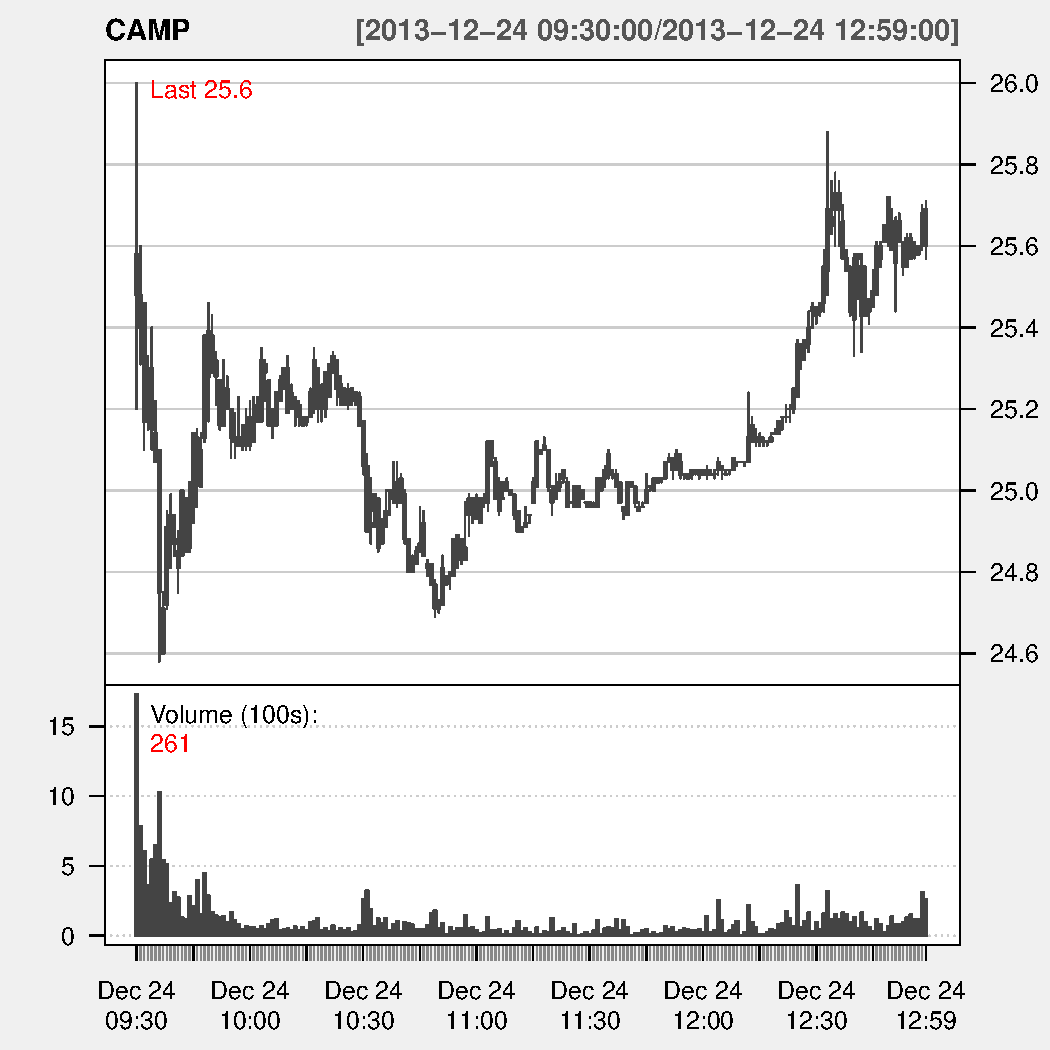
\includegraphics[width=\maxwidth]{/home/jhleong/dev/R/buy_on_gap/BuyOnGap_report/figure/price_chart} 

\end{knitrout}


\end{fullwidth}
\end{document}
